% $Id: experimental.tex 487 2019-01-29 12:15:58Z mspannow $
%
% Basic experimental aspects of jets
%------------------------------------------------------------------------
\section{Experimental aspects}\label{chap:experimental}

The experimental input to the jet algorithms previously discussed is
reconstructed from energy deposits of elementary particles within the
different detector components. The details of the reconstruction
differ between the four LHC experiments, e.g.\ ATLAS uses topoclusters
and CMS uses particle-flow objects as inputs to their jet
recombination algorithms\footnote{ATLAS decided to use particle-flow objects in future studies as well. It will be the default during Run 3 of the LHC.}.
%
While details of how jet constituents are reconstructed can affect the
properties of the jets, we will
constrain our discussion here to a generic description of qualitative
features in the process of measuring them.


\begin{figure}
  \centerline{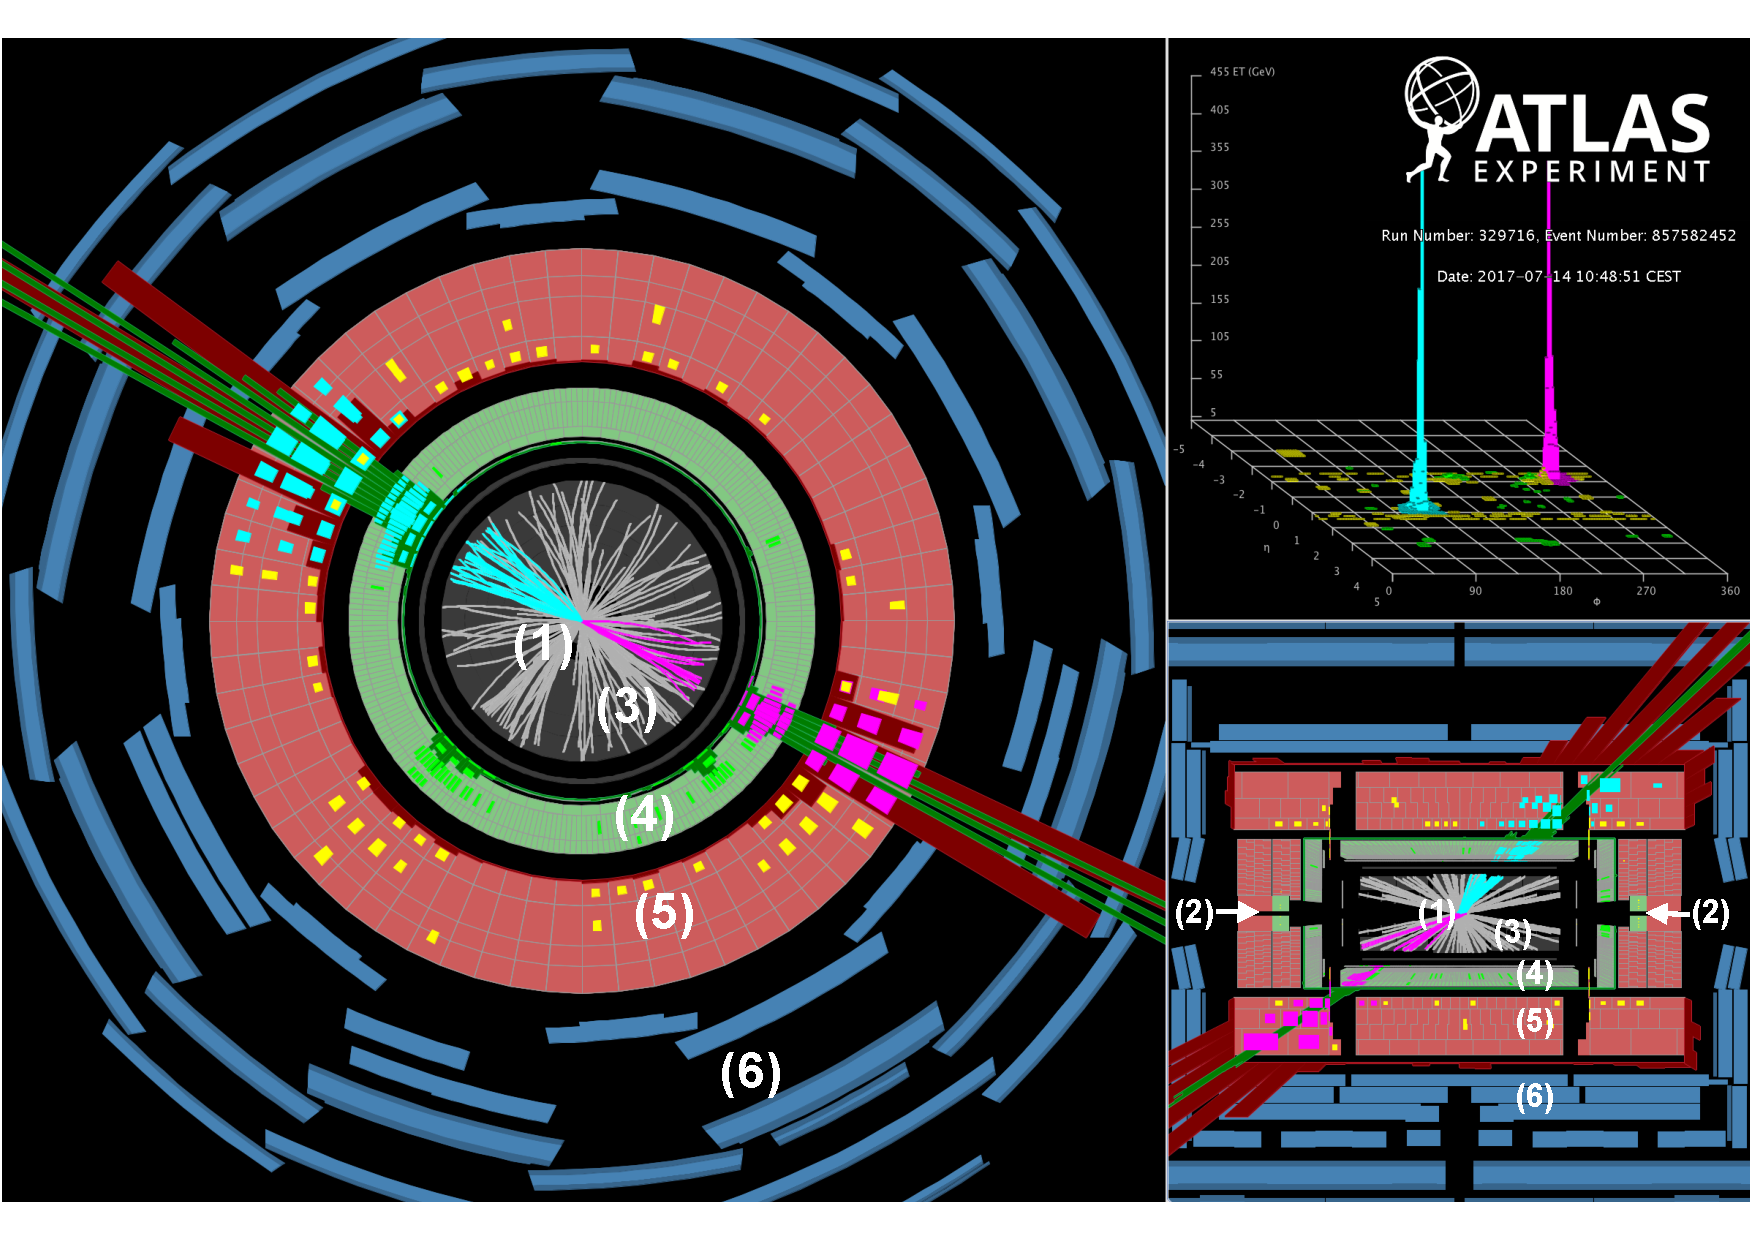
\includegraphics[width=0.90\textwidth]{figures/dijet_event_ATLAS.pdf}}
  \caption{
 Display of a dijet event recorded by ATLAS in proton-proton collisions at centre-of-mass energy 13~TeV. 
The two high-$p_t$ jets have both transverse momentum of 2.9~TeV and the dijet system exhibit an invariant mass of 9.3~TeV. 
The different panels correspond to the view of the event in the plane transverse to the beam direction (large figure on the left-hand side). The two smaller figures on the right-hand side show the calorimeter clusters transverse energies in the $(\eta,\phi)$ plane on the top and the longitudinal view of the event on the bottom. 
The numbers corresponds to different detectors components, as discussed in the text. 
%The figure has been taken and modified from~\cite{dijet-event}.
ATLAS Experiment~\copyright~2018 CERN.}
  \label{fig:detector}
\end{figure}

Multi-purpose detectors at the LHC are cylinder-shaped highly-complex
objects consisting of layers of different components, as depicted in
Fig.~\ref{fig:detector}, each component measuring a certain way a
particle can interact with the detector. Fig.~\ref{fig:detector} shows
a dijet event with an invariant mass of the two jets of $m_{jj} = 9.3$
TeV, measured by ATLAS and consists of three different images. In the
large image on the left the detector plane transverse to the beam axis
is shown. In the lower image on the right we see a lengthwise slice of
the ATLAS detector. The upper image on the right shows the energy
deposits of particles transverse to the beam axis in the so-called
{\it lego-plot} plane. In the lego plot the cylinder shape of the
detector is projected onto a 2-dimensional plane, consisting of the
variables $\eta \in (-\infty, \infty)$, the pseudo-rapidity, cf.\
Eq.~\eqref{eq:def-pseudo-rapidity}, and the azimuthal angle $\phi \in
[0,2 \pi]$.
% 
$\eta$ measures how forward a particle is emitted during the proton-proton interaction. 
Note the similarities between the pseudo-rapidity and the rapidity defined in Eq.~(\ref{eq:def-rapidity}): the two coincide for massless particles. 
%
Distances between two cells or particles $i$ and $j$ on the lego plane are measured via 
\begin{equation}
\Delta R_{ij}^{\text{(detector)}} = \sqrt{(\phi_i - \phi_j)^2 + (\eta_i -\eta_j)^2 }.
\label{eq:dr_eta}
\end{equation}
Note that the topoclusters are assumed massless, i.e. their rapidity equates their pseudo-rapidity. Thus, for detector cells the definitions of Eqs.~(\ref{eq:dr_eta}) and~(\ref{eq:DeltaR-def}) agree.
The different detector components are labelled in Fig.~\ref{fig:detector} in the following way:
\begin{itemize}
\item[(1)] Interaction point of the proton beams.
\item[(2)] The arrows indicate the direction of the particle beams. The proton beams are entering from either side of the detector and exit on the opposite side after crossing at the collision point.
\item[(3)] The innermost part of the ATLAS and CMS detectors consists of the tracking detectors which measure the momentum of charged particles. Strong magnetic fields bend the particles when traversing through the detectors. The way the tracks are bent is indicative of the particle's charge, mass and velocity.
\item[(4)] The electromagnetic calorimeter measures predominantly the energies of electrons and photons. Such particles are stopped and induce a cascade of particles, \emph{a shower}, in the calorimeter. Charged particles can be discriminated from photons by the presence or absence of tracks in the tracking detectors. Cell sizes for this calorimeter vary between the central and forward direction of the detector. In the central part they are roughly $(0.025 \times 0.025)$ in the $\phi-\eta$ plane.
\item[(5)] The hadronic calorimeter measures the energies of hadronic particles, e.g. protons and neutrons. As in the case of the electromagnetic calorimeter, charged hadrons can be discriminated from neutral ones due to their energy loss in the tracking detectors. The cells that make the hadronic calorimeter have in the central region of the detector a size of roughly $(0.1 \times 0.1)$ in the $\phi-\eta$ plane.
\item[(6)] The most outer layer of the detector is the muon spectrometer. Muons, produced with characteristic LHC energies, are weakly interacting with the detector material and are consequently not stopped. However, they may leave tracks in the tracking system, undergo energy loss in the electromagnetic and hadronic calorimeter and may eventually interact with the muon spectrometer. 
\end{itemize}

\begin{figure}
  \centerline{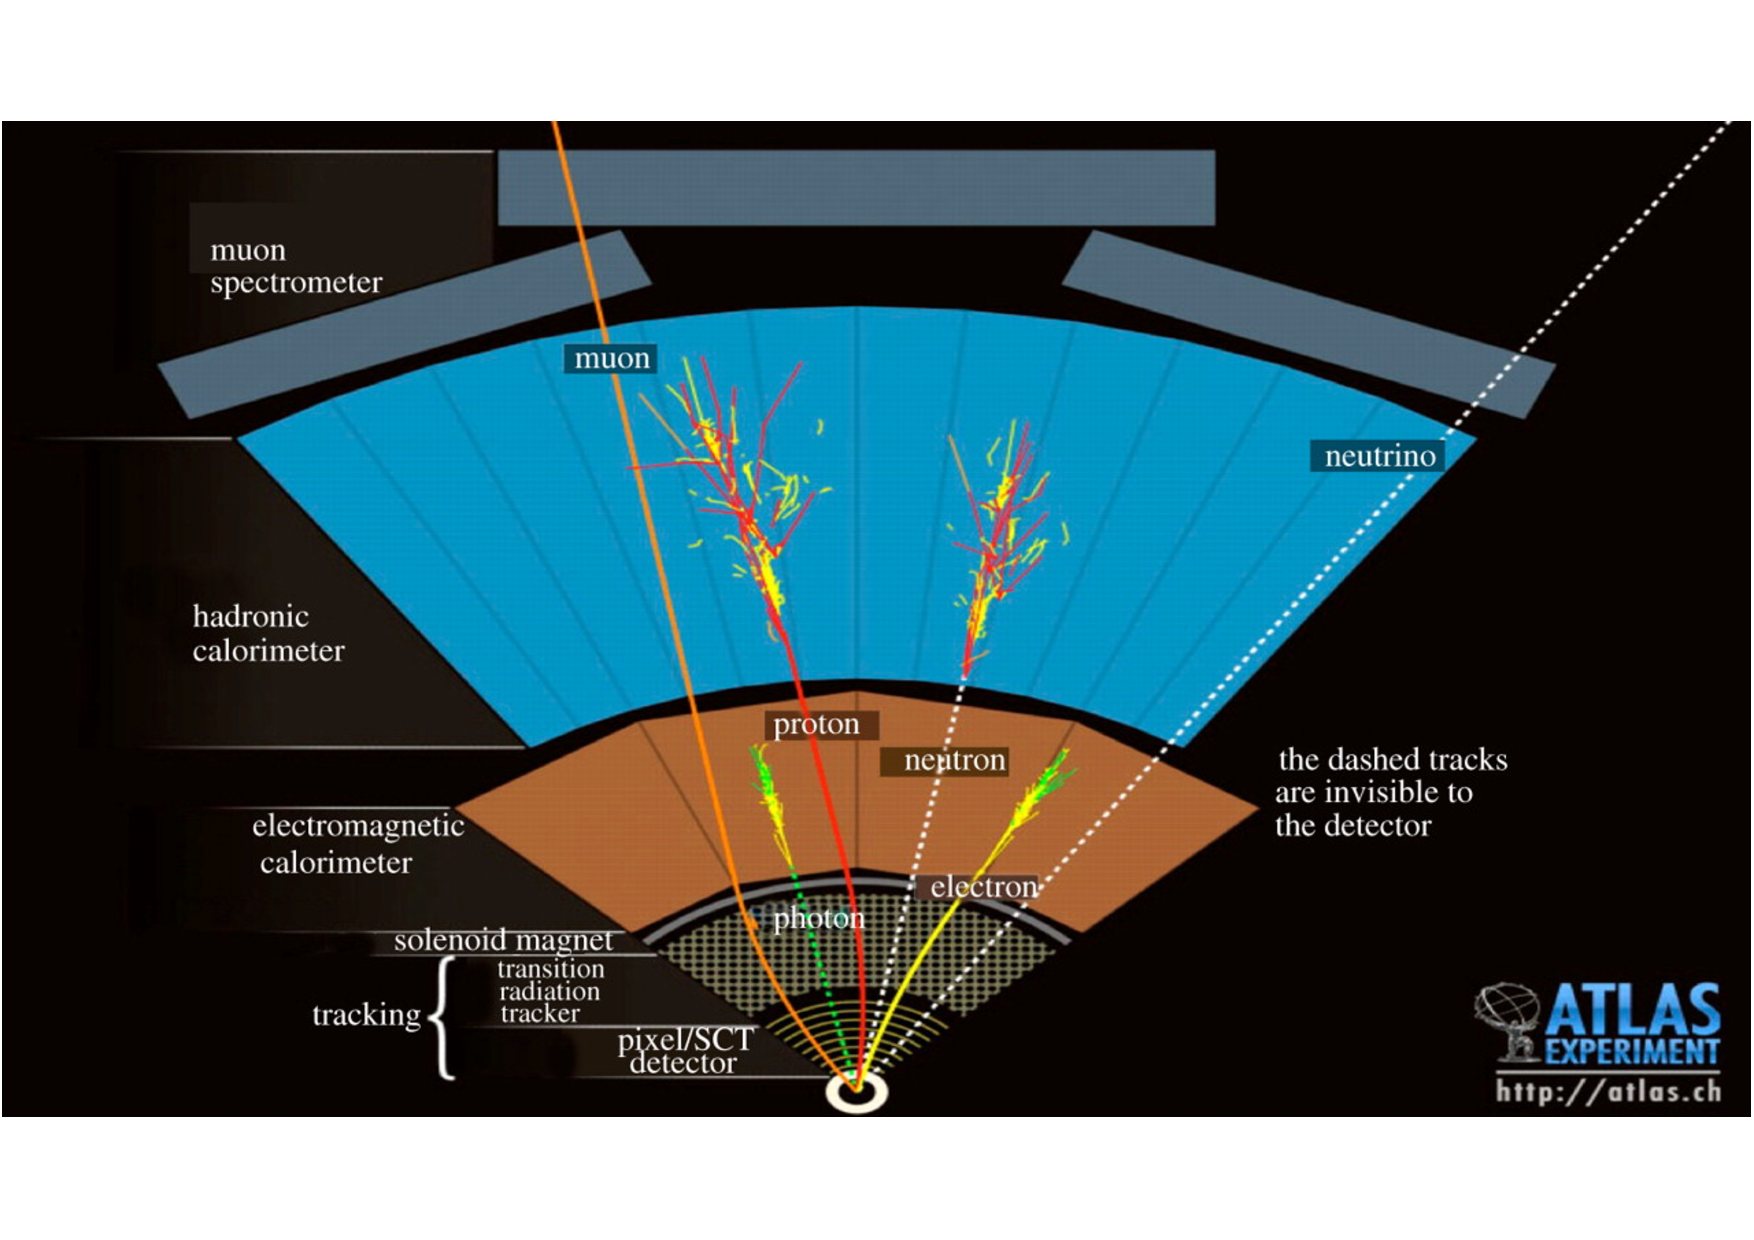
\includegraphics[width=0.95\textwidth]{figures/detector_large.pdf}}
  \caption{Schematic depiction of a multi-purpose detector, here ATLAS. The picture illustrates how different particles interact with the various layers of the detector.  
  ATLAS Experiment~\copyright~2018 CERN.
%  The figure has been taken from Ref.~\cite{Kourkoumelis:2013vpa}).
}
  \label{fig:interaction}
\end{figure}


In Fig.~\ref{fig:interaction} we show a segment of a slice of the transverse plane and how classes of particles interact with the individual detector components. For each high-energy Standard Model event we expect of $\mathcal{O}(500)$ resulting particles, which we can classify into photons, charged leptons, neutral and charged hadrons and non-interacting particles, i.e.\ neutrinos. In a typical proton-proton collision, about 65\% of the jet energy is carried by charged particles, 25\% by photons, produced mainly from $\pi_0$ decays, and only 10\% by neutral hadrons (mostly neutrons and $K_{L} $) \cite{CMS:2010byl, CMS:2010eua}. However, these fractions can vary significantly from event to event.

 
Charged particles loose energy when traversing the detector material in various ways. One mechanism is ionisation and excitation interactions with the detector material, e.g. $\mu^- + \mathrm{atom} \to \mathrm{atom}^* + \mu^- \to \mathrm{atom} + \gamma + \mu^-$, where their energy loss per distance is governed by the Bethe equation \cite{Tanabashi:2018oca}. Further mechanisms for charged particles to interact with the detector material are {\it bremsstrahlung}, {\it direct electron-pair production} and {\it photonuclear interactions
}. 
Photons interact with the detector material through {\it photoelectric effect}, {\it Compton scattering} and {\it electron-pair production}. The latter being dominant for $E_\gamma \gg 1$ MeV.
In the case of hadron-detector interactions, we are dealing mostly with inelastic processes, where secondary strongly interacting particles are produced in the collision.

\vspace{0.3cm}

\begin{wrapfigure}{R}{0.5\textwidth}
 \centering
  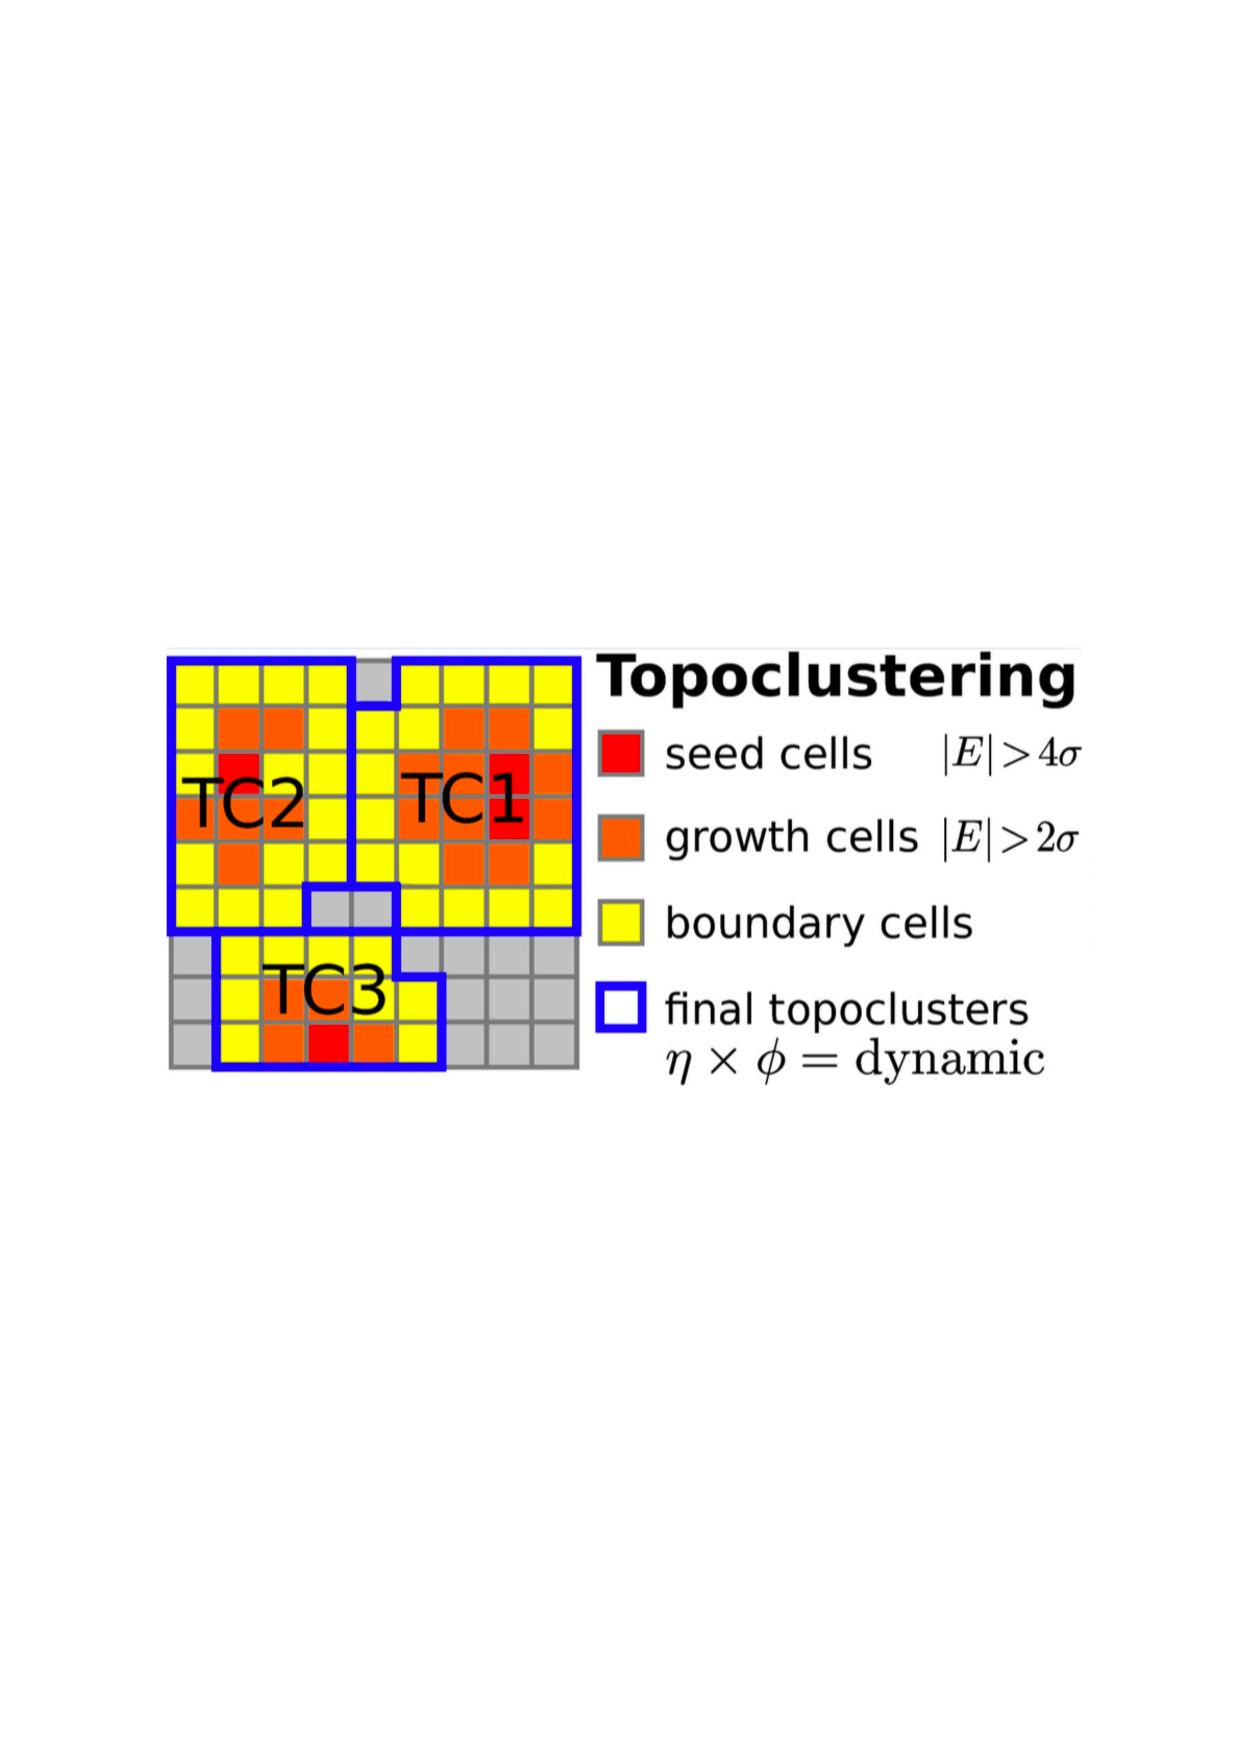
\includegraphics[width=0.5\textwidth]{figures/topocluster.pdf}
  \caption{The figure shows how calorimetric information is used by ATLAS to construct jet constituents (taken from~\cite{boosttalk}).}
  \label{fig:topoclusters}
\end{wrapfigure}

Information gathered from the detector components (3)-(6) allow to
obtain a global picture of the particles produced in the
event. However, particles are not directly used as input to construct
jets using the algorithms previously discussed. ATLAS and CMS use
different approaches to construct jet constituents. The former is
using topological clusters, or, in short, topoclusters, which are
mainly based on calorimeter objects, while the latter use so-called
particle flow objects, which combine information from the tracker and
the calorimeter to build a coherent single object.\footnote{Note that
  ATLAS is moving to using a particle flow approach as well.} The
benefit of using calorimeter objects is a good calibration of the
energy component of the topoclusters. On the other hand, the cell size
of the hadronic calorimeter is $0.1 \times 0.1$ in $(\eta, \phi)$ and
topological cell clusters are formed around seed cells with an energy
$|E_\mathrm{cell}|$ at least $4 \sigma$ above the noise by adding the
neighbouring cells with $|E_\mathrm{cell}|$ at least $2\sigma$ above
the noise, and then all surrounding cells \cite{Aad:2012vm}, see
Fig.~\ref{fig:topoclusters}. The minimal transverse size for a cluster
of hadronic calorimeter cells is therefore $0.3 \times 0.3$ and is
reached if all significant activity is concentrated in one cell. Two
energy depositions leave distinguishable clusters if each one hits
only a single cell and their individual axes are separated by at least
$\Delta R = 0.2$, so that there is one empty cell between the two seed
cells. In the context of this bbok, it means that if important
characteristics of the substructure in a jet are so close that it does
not leave separate clusters in the jet, it is impossible to resolve
it. This leaves a residual lower granularity scale when using
topocluster as fundamental objects to form jets. Thus, in particular
when a fine-grained substructure in the jet is of importance, e.g. in
the reconstruction of highly boosted resonances, the benefit of
particle flow objects is widely appreciated across both multi-purpose
experiments.





Focusing exclusively on the tracking detectors when reconstructing jets is an even more radical approach to optimising the spatial resolution of a final state. Tracking detectors can reconstruct the trajectories of a charged particles, which carry $\sim 65\%$ of the final state's energy, and can specify the direction of the particle at any point of the trajectory with a precision much better than the granularity of the calorimeter. For example, the angular resolution of the ATLAS inner tracking detector for charged particles with $p_T = 10$ GeV and $\eta  = 0.25$ is $\sim 10^{-3}$ in $\eta$ and $\sim 0.3$ mrad in $\phi$ \cite{Aad:2008zzm} with a reconstruction efficiency of $> 78\%$ for tracks of charged particles with $p_T > 500$ MeV \cite{Aad:2010ac}. Further, the momentum resolution for charged pions is 4\% for momenta $|p| < 10$ GeV, rising to 18\% at $|p| = 100$ GeV \cite{Aad:2008zzm}.
%
Note that, generally speaking, the energy resolution tends to degrade
with energy in for calorimeters, but improves with energy for trackers.


%  LocalWords:  topoclusters Eq eq lego Eqs
